\chapter{Problem Definition}

Here, we formally define our system’s optimization goal and discuss the problem’s complexity. Applications provide a set of query templates \(T = \{T_1, T_2, . . .\}\) as the workload specification and a performance goal R. Given the set of query templates T,  system generates trained models for scheduling workloads with queries instances drawn from T. Let us assume a workload \(Q = \{q_1^x , q_2^y , . . . \}\) where each query \(q^j_i \in Q\) is an instance of the template \(T_j \in T\). Given a workload Q and one of the generated decision models, we identify a schedule S for executing Q. We represent a VM of type i, \(vm_i\), as a queue \(vm_i = [q_1^x, q_2^y, . . .]\) of queries to process in that order and we represent a schedule \(S = \{vm_1^i, vm_2^j , . . . \}\) of the workload Q as a list of VMs such that each VM contains only queries from Q. Hence, each schedule S indicates (1) the number and type of VMs to be provisioned, (2) the assignment of each query  \(q_j^ị \in Q\) to these VMs and (3) the query execution order on each VM, \(vm^i_j \in S\). A complete schedule assigns each query in Q to one VM. 

We denote the latency of a query \(q^x_j\) (of template \(T_x\)) when executed on a VM of type i, \(vm^i_k\), as \(l(q^x_j , i)\). Latency estimates can be provided by either the application (e.g., by executing representative queries a-priori on the available VM types) or by using existing prediction models . Queries assigned to a VM can be executed immediately or can be placed in a VM’s processing queue if no more concurrent queries can be processed.
Figure~\ref{fig:Sche} shows two possible schedules for a workload of four queries drawn out of two templates. The first scenario uses three VMs while the second executes the queries on two VMs. Based on our notation, the first schedule is expressed as \(S_1 = \{vm_1 = [q^2_2, q^1_1], vm_2 = [q^2_3], vm_3 = [q^2_4]\}\), where as the second scenario is expressed as \(S_2 = \{vm_1 = [q^1_1, q^2_2], vm_2 = [q^2_3, q^2_4]\}\).
\begin{figure}
\centering
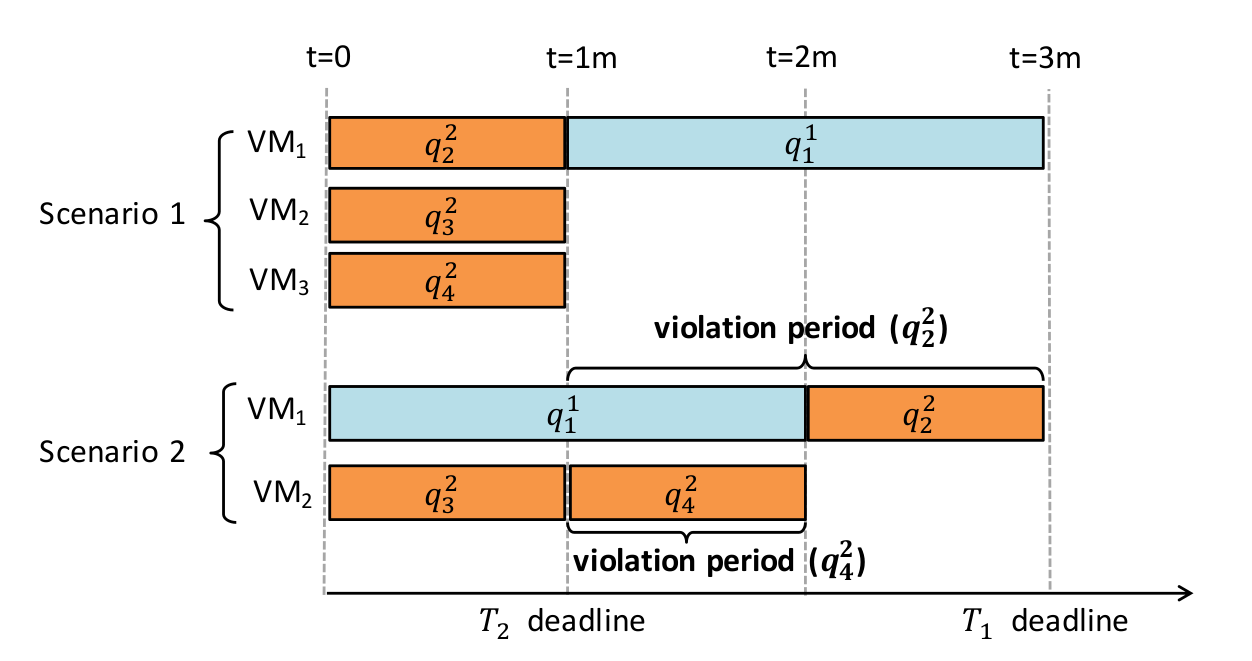
\includegraphics[width=1.0\textwidth]{schedule.png}
\caption{\label{fig:Sche}Two different schedules for a workload}
\end{figure}
\section{Cost Model}
To calculate the monetary cost of processing a workload, we assume each VM of type i has a fixed start-up cost \(f^i_s\), as well as a running cost \(f^i_r\) per unit of time (i.e. the price for renting the VM for that time unit). We also assume a penalty function \(p(R,S)\) that estimates the penalty for a given schedule S and performance goal R. Without loss of generality (and similarly to the model used by IaaS providers), we assume penalties are calculated based on the violation period, i.e., a fixed amount per time period of violation within a schedule S. 

The violation period is the duration of time that the performance goal R was not met. If the goal is to complete queries of a given template within a certain deadline (per query deadline goal), the violation period for each query is measured from the time point it missed its deadline until its completion. Figure~\ref{fig:Sche} shows an example of this case. Let us assume that queries of template \(T_1\) have an execution time of 2 minutes and queries of \(T_2\) execute with 1 minute. The figure shows the violation periods for the second scenario (for \(q^2_2\), \(q^2_4\)) assuming that the deadline of template \(T_1\) is 3 minute and for \(T_2\) is 1 minutes (the first scenario does not have any violations). 

For the maximum latency metric, where no query can exceed the maximum latency, the violation period is computed in the same way. For an average latency performance goal, the duration of the violation period is the difference between the desired average latency and the actual average latency of each query. For a percentile performance goal that requires x\% of queries to be complete in y minutes, the violation period is the amount of time in which 100 - x\% of the queries had latencies exceeding y minutes

\section{Problem Definition}
Given a workload \(Q = \{q_1^x , q_2^y , . . . \}\), where \(q^j_i\) is of template \(T_j\) , and a performance goal R, our goal is to find a complete schedule S that minimizes the total monetary cost (provisioning, processing, and penalty payouts costs) of executing the workload. We define this total cost, \(cost(R, S)\), as 
\begin{equation} \label{eq:1}
cost(R,S) =  \sum_{vm^i_j \in S} [f^i_s + \sum_{q^m_k \in vm^i_j} (f^i_r \times l(q^m_k,i))] + p(R,S)
\end{equation}

\section{Problem Complexity}
Under certain conditions, our optimization problem becomes the bin packing problem, where we try to “pack” each query into one of the available “VM-bins”. For this reduction, we need to assume that the number of query templates is unbounded, infinite penalty, \(p(R, S) = \infty\), if the performance goal is violated, and the start-up cost \(f^i_s\) is uniform across all VM types. Under these conditions, the problem is NP-Hard. However, these assumptions are not valid in our system. Limiting the number of query templates relaxes the problem to one of polynomial complexity, but still not computationally feasible. 

Two common greedy approximations to this optimization problem are the first-fit decreasing (FFD) and first-fit-increasing (FFI) algorithms, which sort queries in decreasing or increasing order of latency respectively and place each query on the first VM where the query “fits” (incurs no penalty). If the query will not fit on any VM, a new VM is created. Existing cloud management systems have used FFD  for provisioning resources and scheduling queries. However, it is often not clear which of these greedy approaches is the best for a specific workload and performance goal. For example, when applied to the workload and performance goals shown in Figure 2, FFD schedules all queries on their own VM, which offers the same performance as scenario 1 but uses an additional VM (and hence has higher cost). A better approximation would be FFI, which produces the schedule that is depicted in scenario-1, scheduling the four queries across three VMs without violating the performance goal. 

Furthermore, there might be scenarios when none of these approximations offer the best solution. For example, consider workloads consisting of three templates, \(T_1, T_2, T_3\) with latencies of four, three, and two minutes respectively. Assume we have two queries of each template, \(q^1_1, q^1_2\) of template \(T_1\), \(q^2_3, q^2_4\) of template \(T_2\), and \(q^3_5, q^3_6\) of template \(T_3\) and we wish to keep the total execution time of the workload below nine minutes. FFD will find the schedule \(S_{FFD} = \{[ q^1_1, q^1_2], [q^2_3, q^2_4, q^3_5], [q^3_6]\}\), while FFI would find the schedule \(S_{FFI} = \{q^3_5, q^3_6, q^2_3], [q^2_4, q^1_1], [q^1_2]\}\). However, a better strategy is one that attempts to place an instance of T1, then an instance of T2, then an instance of T3, then create a new VM, resulting in the schedule \(S_1 = \{[q^1_1, q^2_3, q^3_5], [q^1_2, q^2_4, q^3_6]\}\), which has a lower cost because it provisions one less VM. 

Our system departs from the “one-strategy-fits-all” approach used by standard approximation heuristics. Instead, it offers effective scheduling strategies for custom performance goals and workload specifications by learning heuristics tailored to the application’s needs. We next describe how we identify such strategies.
